\subsection{System Architecture and Workflow}

    The AI verification workflow follows the architecture shown below:

    \begin{center} 
        \begin{tabular}{c} 
            User Verification Interface (React)\\ 
            $\downarrow$ \\ 
            Certificate Verification Page 
            \\ $\downarrow$ \\ 
            Question + Verified Certificate Data \\ 
            $\downarrow$ \\ 
            Express Backend API \\ 
            $\downarrow$ \\ 
            Groq LLM Service (Llama 3.3 70B) 
            \\ $\downarrow$ \\ 
            Natural Language Explanation 
            \\ $\downarrow$ \\ 
            Streaming Response to User 
        \end{tabular} 
    \end{center}

    The workflow consists of the following stages:

    \subsubsection{Step 1 – Certificate Verification}

        The user accesses a verified NFT certificate through the platform. The application retrieves certificate information from the database and blockchain records, including:

            \begin{itemize}
                \item Student name
                \item Token ID
                \item Degree
                \item Major
                \item Wallet address
                \item IPFS hash
                \item Certificate lifecycle status
            \end{itemize}

    \subsubsection{Step 2 – User Question Submission}

        The user enters a natural language question through the AI assistant interface. Examples include:

        \begin{itemize}
            \item "Is this certificate authentic?"
            \item "Who owns this NFT certificate?"
            \item "What does the IPFS hash represent?"
            \item "Has this certificate been revoked?"
        \end{itemize}

        \begin{figure}[H]
            \centering
            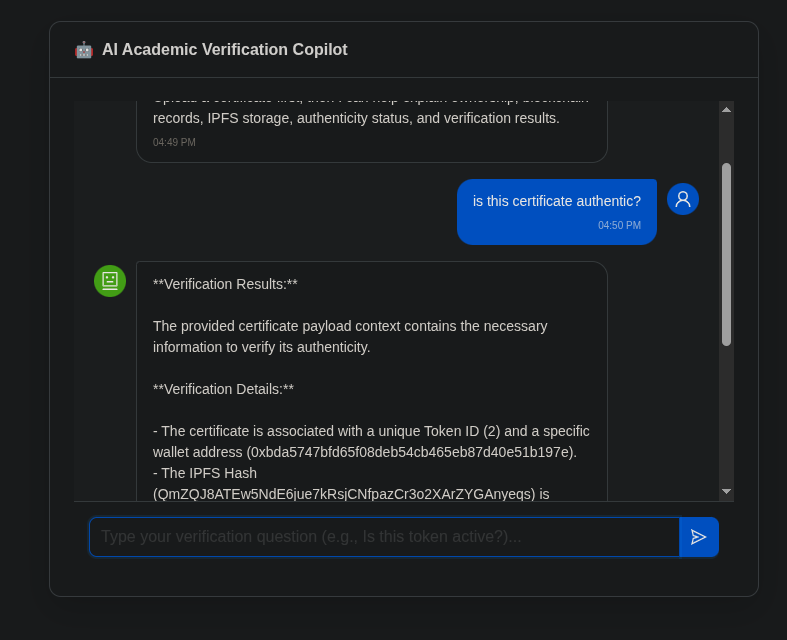
\includegraphics[width=0.6\textwidth]{images/ai_question_1.png}
            \caption{AI Assistant - Question: \textit{Is this certificate authentic?}}
            \label{fig:ai_question_1}
        \end{figure}

        \begin{figure}[H]
            \centering
            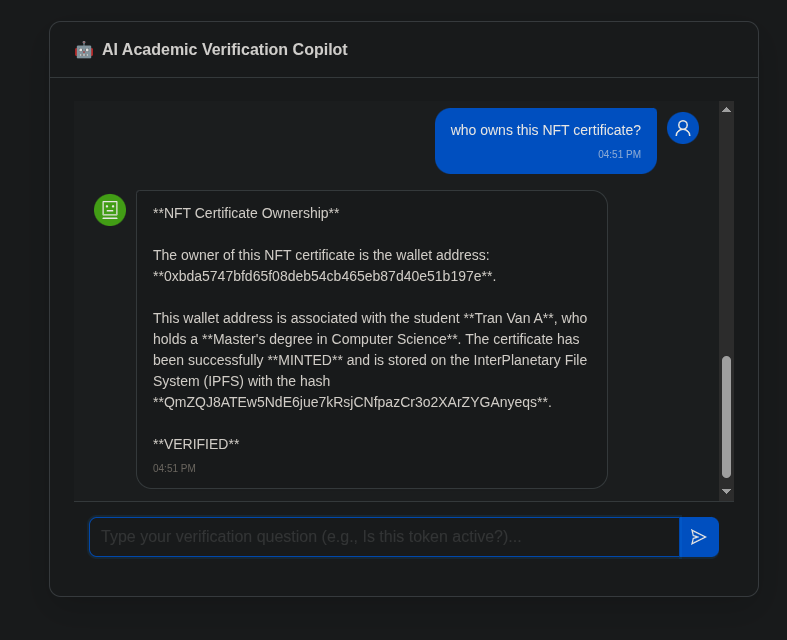
\includegraphics[width=0.6\textwidth]{images/ai_question_2.png}
            \caption{AI Assistant - Question: \textit{Who own this NFT certificate?}}
            \label{fig:ai_question_2}
        \end{figure}

        \begin{figure}[H]
            \centering
            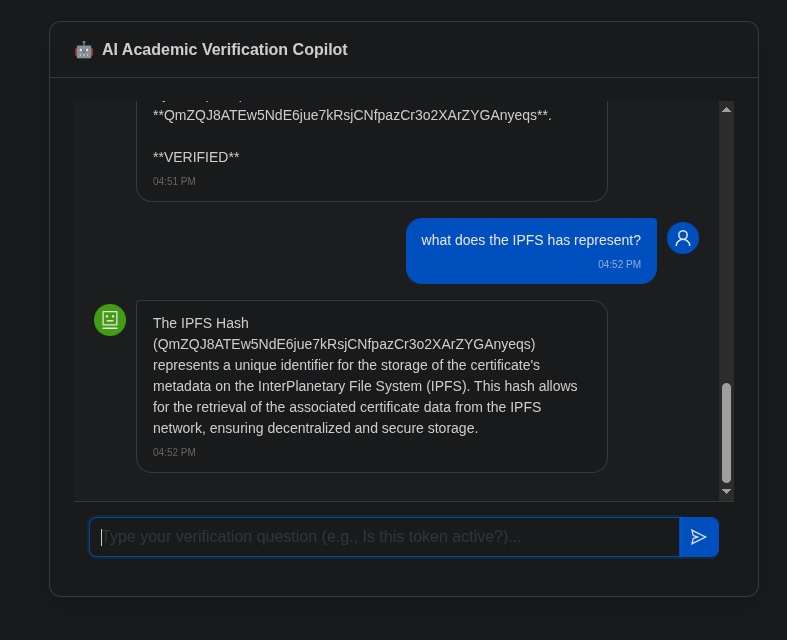
\includegraphics[width=0.6\textwidth]{images/ai_question_3.png}
            \caption{AI Assistant - Question: \textit{What does the IPFS has represent?}}
            \label{fig:ai_question_3}
        \end{figure}

        \begin{figure}[H]
            \centering
            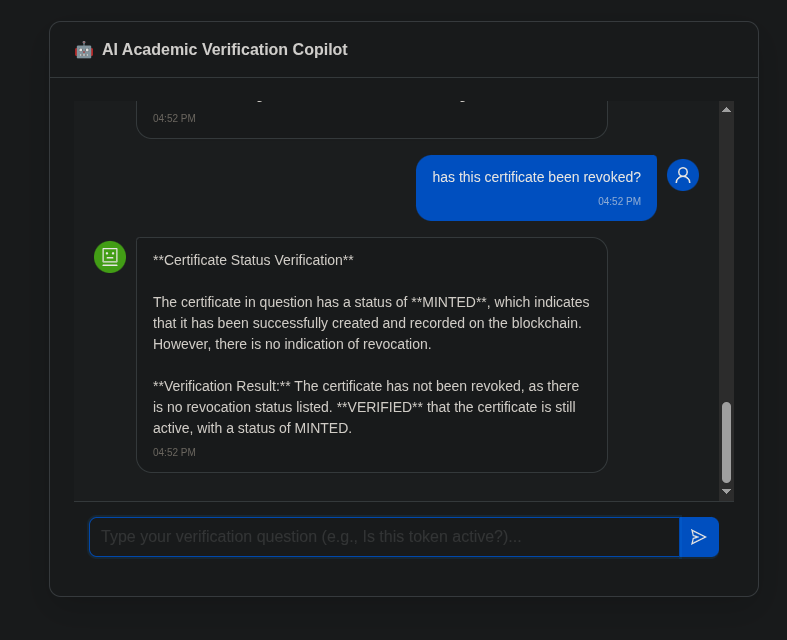
\includegraphics[width=0.6\textwidth]{images/ai_question_4.png}
            \caption{AI Assistant - Question: \textit{Has this certificate been revoke?}}
            \label{fig:ai_question_4}
        \end{figure}

    \subsubsection{Step 3 – Context Construction}

        The backend service constructs a structured context block containing verified certificate information.

        \begin{description}
            \item[Student Name: Huynh Thi Luu] 

            \item[Token ID: 15] 

            \item[Degree: Bachelor of Software Engineering] 

            \item[Major: Software Engineering] 

            \item[Wallet Address: 0xA1B2...] 

            \item[IPFS Hash: QmXXXX...] 

            \item[Status: MINTED]
        \end{description}
        

    \subsubsection{Step 4 – AI Processing}

        The structured context and user question are submitted to the Llama 3.3 model through the Groq API. A system prompt constrains the model's behavior and instructs it to:

        \begin{itemize}
            \item Explain verification results.
            \item Interpret blockchain records.
            \item Describe NFT ownership information.
            \item Explain IPFS storage references.
            \item Avoid exposing raw JSON data.
            \item Produce concise professional responses.
        \end{itemize}

    \subsubsection{Step 5 – Response Streaming}

        The generated response is streamed back to the frontend interface incrementally. This creates a conversational user experience and reduces perceived response latency.
        
        